\chapter[Общие сведения о библиотеке MathGL]{Общие сведения о библиотеке MathGL}
При решении различных задач, возникает необходимости графического отображения данных (графики, диаграммы, поверхности).
Одним из универсальных способов построения различных графиков является кросс-платформенная библиотека \Sys{MathGL}.

\index{Библиотека!MathGL}\Sys{Mathgl} --- свободная кросс-платформенная библиотека для построения 2-х и 3-х
мерных графиков функций. Её использование позволит построить график с помощью нескольких операторов. Синтаксис функций,
используемых в \Sys{MathGL}, подобен синтаксису \Sys{MathLab, Octave, Scilab, GnuPlot}. Официальный сайт --- 
\url{http://mathgl.sourceforge.net/doc_ru/Website.html#Website}, на странице загрузки
\url{http://mathgl.sourceforge.net/doc_ru/Download.html#Download} можно скачать последнюю версию программы для различных
операционных систем, англоязычную документацию в формате pdf. Группа в Google --- \url{https://groups.google.com/forum/#!forum/mathgl}.
Русскоязычная страница с описанием --- \url{http://mathgl.sourceforge.net/doc_ru/index.html#SEC_Contents}, англоязычная ---
\url{http://mathgl.sourceforge.net/doc_en/index.html#SEC_Contents}. Кроме \Sys{С(С++)} поддерживаются \Sys{Fortran, Python, Octave}, скриптовый язык \Sys{MGL}.

Рассмотрим особенности установки и примеры использования библиотеки для построения графиков.

\section{Установка MathGL в Linux.}
Библиотека входит в репозитории большинства современных дистрибутивов Linux. Её можно установить из репозитория
стандартным для вашего дистрибутива, однако в репозитории зачастую находится не самая новая версия. Для установки самой
новой версии необходимо:

\begin{enumerate}
\item Скачать исходники последней версии с официального сайта.
\item Распаковать.
\item Последовательно выполнить команды\footnote{Перед выполнением команды \Sys{cmake}, возможно, придётся доставлять
необходимые пакеты. При работе в debian (6, 7), ubuntu (12.04, 12.10, 13.04, 13.10) авторам пришлось доставить  пакеты
\Sys{cmake, zlib1g-dev, libpng12-dev, libqt4-opengl-dev, libqtwebkit-dev}. Кроме того, должен быть устанвлен компилятор \Sys{g++}.}
\begin{verbatim}
cmake -Denable-qt=ON
cmake
make
sudo make install
\end{verbatim}
\item Скопировать файлы \Sys{libmgl-qt.so.7.1.0} и \Sys{libmgl.so.7.1.0}\footnote{Версии библиотек \Sys{libmgl} 
указаны применительно к mathgl 2.2, в вашем конкретном случае могут быть другие библиотеки.} 
из каталога \Sys{/usr/local/lib} в каталог \Sys{/lib} (нужны права администратора(суперпользователя)).
\end{enumerate}

После этого для компиляции программы с использованием библиотеки \Sys{MathGL} необходимо использовать ключи \Sys{-L/usr/local/lib -L/usr/lib -lmgl -lmgl-qt}, например для компиляции файла с именем \Sys{1.cpp} можно использовать команду
\begin{verbatim}
g++ -o 1  1.cpp -L/usr/local/lib -L/usr/lib -lmgl -lmgl-qt
\end{verbatim}

Рассмотрим возможности библиотеки на конкретных примерах.

\prg{Построить график функции  $f(x)=\sin (x)+\frac{1}{3}\cdot
\sin (3\cdot x)+\frac{1}{5}\cdot \sin (5\cdot x)$.}{appb:prg0}

Следующий программный код позволит построить линию графика (рис.~\ref{appb:refDrawing0}) на интервале $[-1;1]$.
\begin{lstlisting}
#include <mgl2/qt.h>
int sample(mglGraph *gr)
{
  gr->Title("`\Sys{График функции}` y=f(x)"); //`Заголовок графика`
  //`График заданной функции. Линия графика изображена красным цветом --- `"r".
  gr->FPlot("sin(x)+1/3*sin(3*x)+1/5*sin(5*x)","r");
  return 0;
}
int main(int argc,char **argv)
{
  setlocale(LC_CTYPE, "ru_RU.utf8");
  mglQT gr(sample,"Plot");
  return gr.Run();
}
\end{lstlisting}

Далее представлен текст программы, с помощью которого можно усовершенствовать график, показанный на рис.~\ref{appb:refDrawing0}. 
На рис.~\ref{appb:refDrawing1} видно, что был увеличен диапазон построения графика, добавлены оси координат,
подписи под ними и линии сетки.

\begin{figure}[htb]
\begin{center}
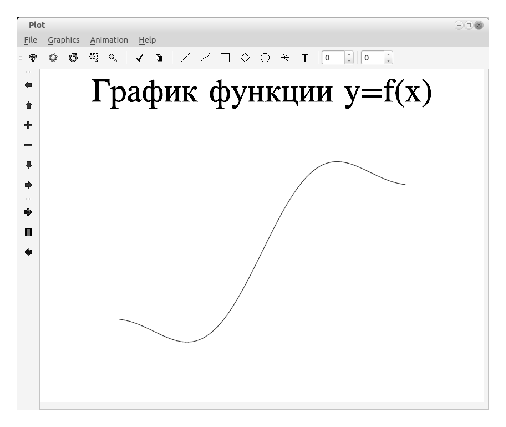
\includegraphics[width=0.7\textwidth]{img/ris_appb_1}
\caption{График функции к задаче \ref{appb:prg0}}
\label{appb:refDrawing0}
\end{center}
\end{figure}

\begin{lstlisting}
#include <mgl2/qt.h>
int sample(mglGraph *gr)
{
  gr->Title("`\Sys{График функции}` y=f(x)"); //`Заголовок графика`
  gr->SetOrigin(0,0); //`Установка центра координатных осей`
  //`Границы по оси абсцисс от -10 до 10, по оси ординат от -1 до 1.`
  gr->SetRanges(-10,10,-1,1);
  gr->Axis(); //`Вывод значений возле осей`
  gr->Grid(); //`Линии сетки`
  //`График заданной функции.`
  gr->FPlot("sin(x)+1/3*sin(3*x)+1/5*sin(5*x)", "r");
  return 0;
}
int main(int argc,char **argv)
{
  setlocale(LC_CTYPE, "ru_RU.utf8"); //`Поддержка кириллицы в С++`
  mglQT gr(sample,"Plot"); //`Вывод графика на экран в окно с именем Plot`
  return gr.Run();
}
\end{lstlisting}

\begin{figure}[htb]
\begin{center}
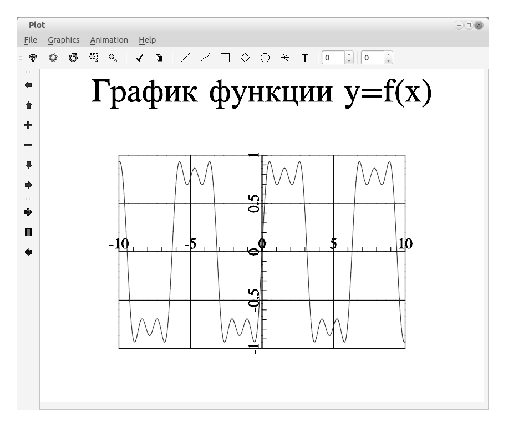
\includegraphics[width=0.7\textwidth]{img/ris_appb_2}
\caption{Форматирование линии и области построения графика к задаче \ref{appb:prg0}}
\label{appb:refDrawing1}
\end{center}
\end{figure}

\prg{Построить графики функций  $f(x)=\sin (2\cdot x)$ и 
$y(x)=\frac{4\cdot \cos (x)}{3}$  в одной графической области.}{appb:prg1}

Далее приведен текст программы реализующий решение поставленной задачи. Результаты работы программы показаны на рис.
\ref{appb:refDrawing2}.
\begin{lstlisting}
#include <mgl2/qt.h>
#include <math.h>
int sample(mglGraph *gr)
{  
  gr->Title("`\Sys{Графики функции}` y=f(x)"); //`Заголовок графика`
  gr->SetRanges(-15,15,-2,2); //`Границы по осям`
  gr->Axis(); //`Вывод значений возле осей`
  gr->Grid(); //`Линии сетки`
  gr->FPlot("sin(2*x)", "r"); //`График функции f(x), красная (r) сплошная линия.`
  gr->AddLegend("sin(2*x)","r"); //`Добавление легенды`
  gr->FPlot("4*cos(x)/3", "k."); //`График функции y(x), чёрная (k) линия и точки (.).`
  gr->AddLegend("4*cos(x)/3","k."); //`Добавление легенды`
  gr->Legend(3); //`Вывод легенды на экран в правом верхнем углу`
  gr->Label('x',"OX",0); //`Вывод подписи по оси абсцисс`
  gr->Label('y',"OY"); //`Вывод подписи по оси ординат`
  return 0;
}
int main(int argc,char **argv)
{
  setlocale(LC_CTYPE, "ru_RU.utf8");
  mglQT gr(sample,"Plot");
  return gr.Run();
}
\end{lstlisting}

\begin{figure}[htb]
\begin{center}
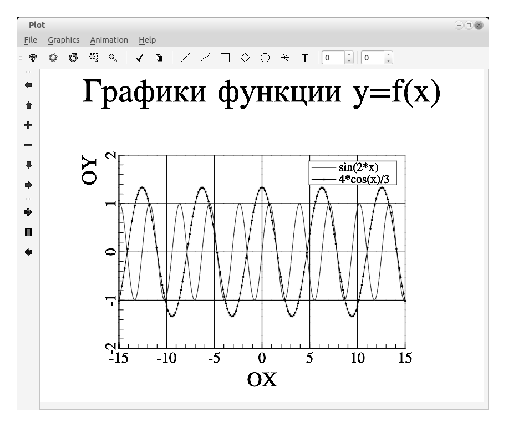
\includegraphics[width=0.7\textwidth]{img/ris_appb_3}
\caption{Графики к задаче \ref{appb:prg1}}
\label{appb:refDrawing2}
\end{center}
\end{figure}

\prg{Построить в одном графическом окне графики функций:}{appb:prg2}

\begin{itemize}
\item  $f(x)=\sin (x)$ на интервале $[-10;10]$, 
\item  $f(x)=\cos (x)$ на интервале $[-6;6]$, 
\item  $f(x)=e^{\cos (x)}$ на интервале $[-6;6]$,
\item  $f(x)=e^{\sin (x)}$ на интервале $[-12;12]$.
\end{itemize}
Результаты вывести на экран и в файл.

Далее приведен программный код и результат его работы (рис. \ref{appb:refDrawing3}).
\begin{lstlisting}
#include <mgl2/qt.h>
#include <mgl2/mgl.h>
#include <iostream>
using namespace std;
int sample(mglGraph *gr)
{
  //`График функции $\sin (x)$ на интервале $[-10;10]$`
  gr->SubPlot(2,2,0); 
  gr->Title("`\Sys{График функции}` sin(x)");
  gr->SetOrigin(0,0);
  gr->SetRanges(-10,10,-1,1);
  gr->Axis(); 
  gr->Grid(); 
  gr->FPlot("sin(x)","k-.");
  //`График функции $\cos (x)$ на интервале $[-6;6]$`
  gr->SubPlot(2,2,1); 
  gr->Title("`\Sys{График функции}` cos(x)");
  gr->SetOrigin(0,0);
  gr->SetRanges(-6,6,-1,1);
  gr->Axis(); 
  gr->Grid(); 
  gr->FPlot("cos(x)","k .");
  //`График функции $\exp (\cos (x))$ на интервале $[-6;6]$`
  gr->SubPlot(2,2,2);
  gr->Title("`\Sys{График функции}` e^{cos(x)}");
  gr->SetOrigin(0,0);
  gr->SetRanges(-6,6,0,3);
  gr->Axis(); 
  gr->Grid(); 
  gr->FPlot("exp(cos(x))","r o");
  //`График функции $\exp (\sin (x))$ на интервале $[-12;12]$`
  gr->SubPlot(2,2,3); 
  gr->Title("`\Sys{График функции}` e^{sin(x)}");
  gr->SetOrigin(0,0);
  gr->SetRanges(-15,15,0,3);
  gr->Axis(); 
  gr->Grid(); 
  gr->FPlot("exp(sin(x))","r-o");
  return 0;
}
int main(int argc,char **argv)
{
  //`Вывод на экран или в файл`
  int k;
  cout<<"`\Sys{Введите 1, если будете выводить на экран, 2 - если в файл}`\nk=";
  cin>>k;
  if(k==1)
  {
    //`Поддержка кириллицы в С++`  
    setlocale(LC_CTYPE, "ru_RU.utf8");
    //`Вывод на экран`
    mglQT gr(sample,"Plots");
      return gr.Run();
  }
  else
  {
    mglGraph gr;
    gr.Alpha(true);
    gr.Light(true);
    setlocale(LC_CTYPE, "ru_RU.utf8");
    //`Обращение к функции вывода`
    sample(&gr);
    //`Запись изображения в файл`
    gr.WriteEPS("test.eps");
    return 0;
  }
}
\end{lstlisting}

\begin{figure}[htb]
\begin{center}
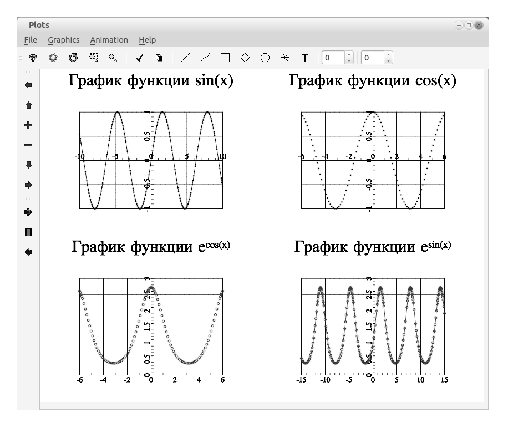
\includegraphics[width=0.7\textwidth]{img/ris_appb_4}
\caption{График функций к задаче \ref{appb:prg2}}
\label{appb:refDrawing3}
\end{center}
\end{figure}

\prg{Построить график функций 
$f(x)=1-\frac{0.4}{x}+\frac{0.05}{x^{2}}$.}{appb:prg3}

Не трудно заметить, что функция \emph{f}(\emph{x}) не существует в точке ноль. Поэтому
построим её график на двух интервалах [-2;-0.1] и [0.1;2], исключив точку разрыва из диапазона построения. Текст
программы с подробными комментариями приведен далее. Решение задачи представлено на рис. \ref{appb:refDrawing4}.
\begin{lstlisting}
#include <mgl2/qt.h>
#include <iostream>
using namespace std;
int sample(mglGraph *gr)
{  
  mglData x1(191),x2(191), y1(191), y2(191) ;
  int i; float h,a1,b1,a2,b2;
  //`График точечной разрывной функции`
  //`Первый интервал`
  a1=-2;b1=-0.1;
  h=0.01;
  for(i=0;i<191;i++)
  {
    x1[i]=a1+i*h;
    y1[i]=1-0.4/x1[i]+0.05/x1[i]/x1[i];
  }
  //`Второй интервал`
  a2=0.1;b2=2;
  h=0.01;
  for(i=0;i<191;i++)
  {
    x2[i]=a2+i*h;
    y2[i]=1-0.4/x2[i]+0.05/(x2[i]*x2[i]);
  }
  gr->SetRanges(a1,b2,0,10); //`Границы по оси абсцисс и ординат`
  gr->Axis(); //`Оси координат`
  gr->Grid(); //`Сетка`
  gr->Plot(x1,y1,"k"); //`График функции на первом интервале, чёрный (k) цвет.`
  gr->Plot(x2,y2,"k"); //`График функции на втором интервале, чёрный (k) цвет.`
  gr->SetFontSize(2); //`Размер шрифта`
  gr->Title("`\Sys{График разрывной функции}`"); //`Заголовок`
  gr->SetFontSize(4); //`Размер шрифта`
  gr->Label('x',"OX",0); //`Подпись по оси абсцисс`
  gr->Label('y',"OY"); //`Подпись по оси ординат`
return 0;
}
int main(int argc,char **argv)
{
  setlocale(LC_CTYPE, "ru_RU.utf8");
  mglQT gr(sample,"Plot");
  return gr.Run();
}
\end{lstlisting}

\begin{figure}[htb]
\begin{center}
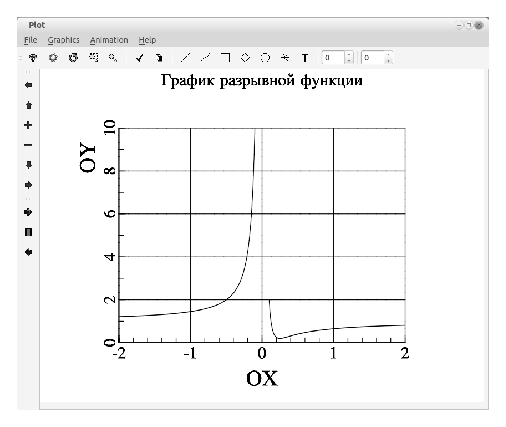
\includegraphics[width=0.7\textwidth]{img/ris_appb_5}
\caption{График функции к задаче \ref{appb:prg3}}
\label{appb:refDrawing4}
\end{center}
\end{figure}


\prg{Построить график функции  $x(t)=3\cdot \cos (t),y(t)=2\cdot\sin (t)$.}{appb:prg4}

График задан в параметрической форме и представляет собой эллипс. Выберем интервал построения графика  $[0;2\cdot \pi
]$, ранжируем переменную \emph{t} на этом интервале, сформируем массивы \emph{x} и
\emph{y} и построим точечный график. Текст программы и результаты ее работы (рис. \ref{appb:refDrawing5})
представлены далее.
\begin{lstlisting}
#include <mgl2/qt.h>
#include <iostream>
#include <math.h>
using namespace std;
int sample(mglGraph *gr)
{ //`График эллипса`
  int i,n; float h,a,b,t;
  a=0;
  b=2*M_PI;
  n=200;
  h=(b-a)/n;
  //`Формирование массивов абсцисс и ординат`
  mglData x(n),y(n);
  for(i=0;i<n;i++)
  {
    t=a+i*h;
    x[i]=3*cos(t);
    y[i]=2*sin(t);
  }
  gr->SetRanges(-3,3,-2,2); //`Границы по осям координат`
  gr->Axis(); //`Оси координат`
  gr->Grid(); //`Сетка`
  gr->Plot(x,y,"k"); //`График функции`
  gr->SetFontSize(2);
  gr->Title("`\Sys{График эллипса}`");
  gr->SetFontSize(4);
  gr->Label('x',"OX",0);
  gr->Label('y',"OY");
return 0;
}
int main(int argc,char **argv)
{
  setlocale(LC_CTYPE, "ru_RU.utf8");
  mglQT gr(sample,"Plot");
  return gr.Run();
}
\end{lstlisting}

\begin{figure}[htb]
\begin{center}
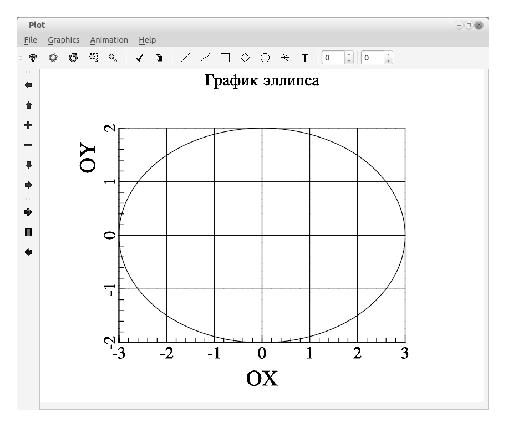
\includegraphics[width=0.7\textwidth]{img/ris_appb_6}
\caption{График к задаче \ref{appb:prg4}}
\label{appb:refDrawing5}
\end{center}
\end{figure}

\prg{Построить график функции:\\
 $z(x,y)=0.6\cdot\sin (2\cdot\pi\cdot x)\cdot\cos (3\cdot\pi\cdot y)+0.4\cdot\cos (3\cdot\pi\cdot x\cdot y)$.}
{appb:prg5}

В данном случае необходимо построить график функции двух аргументов. Для этого нужно сформировать матрицу $z$ при
изменении значений аргументов $x$ и $y$ и отобразить полученные результаты.

Далее приведен текст программы и результаты ее работы (рис. \ref{appb:refDrawing6}).
\begin{lstlisting}
#include <mgl2/qt.h>
#include <iostream>
using namespace std;
int sample(mglGraph *gr)
{
  //`Изображение поверхности`
  gr->SetRanges(-5,5,-5,5,-1,2); //`Диапазон изменения x, y, z.`
  mglData z(500,400); //`Размер матрицы z по х и по y`
  //`Формирование матрицы z.`
  z.Modify("0.6*sin(2*pi*x)*sin(3*pi*y) + 0.4*cos(3*pi*(x*y))");
  gr->Rotate(40,60); //`Вращение осей`
  gr->Box(); 
  gr->Axis(); 
  gr->Grid();
  gr->Mesh(z); //`График функции`
}
int main(int argc,char **argv)
{
  setlocale(LC_CTYPE, "ru_RU.utf8");
  mglQT gr(sample,"MathGL example");
  return gr.Run();
}
\end{lstlisting}

\begin{figure}[htb]
\begin{center}
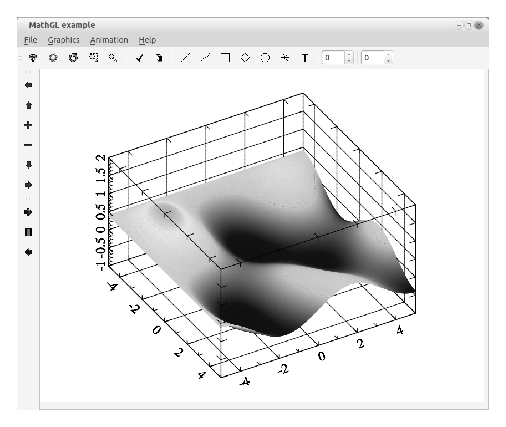
\includegraphics[width=0.7\textwidth]{img/ris_appb_7}
\caption{График к задаче \ref{appb:prg5}}
\label{appb:refDrawing6}
\end{center}
\end{figure}

\prg{Построить эллипсоид.}{appb:prg6}

Текст программы и результаты её работы (рис.~\ref{appb:refDrawing7}).
\begin{lstlisting}
#include <mgl2/qt.h>
#include <mgl2/mgl.h>
#include <iostream>
using namespace std;
int sample(mglGraph *gr)
{  
  gr->Title("`\Sys{Эллипсоид}`");
  mglData x(50,40),y(50,40),z(50,40);
  gr->Fill(x,"0.1+0.8*sin(2*pi*x)*sin(2*pi*y)");
  gr->Fill(y,"0.15+0.7*cos(2*pi*x)*sin(2*pi*y)");
  gr->Fill(z,"0.2+0.6*cos(2*pi*y)");
  gr->Rotate(50,60);
  gr->Box();
  gr->Surf(x,y,z,"BbwrR");
  return 0;
}
int main(int argc,char **argv)
{  
  setlocale(LC_CTYPE, "ru_RU.utf8");
  mglQT gr(sample,"Ellipse");
  return gr.Run();
}
\end{lstlisting}


\begin{figure}[htb]
\begin{center}
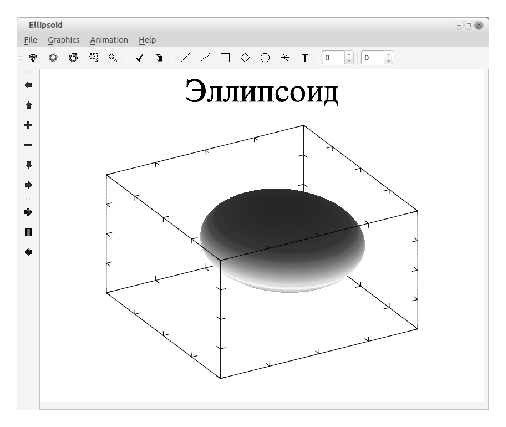
\includegraphics[width=0.7\textwidth]{img/ris_appb_8}
\caption{График к задаче \ref{appb:prg6}}
\label{appb:refDrawing7}
\end{center}
\end{figure}

Для изучения всех возможностей \Sys{MathGL}, авторы советуют обратиться к документации по \Sys{MathGL}. 
При освоении библиотеки \Sys{MathGL} следует помнить, что логика и синтаксис библиотеки напоминает 
синтаксис \Sys{Scilab} и  \Sys{Octave}.

